\documentclass[a4paper, oneside, openany, dvipdfmx]{suribt}% 本文が * ページ以下のときに (掲示に注意)
\usepackage{graphicx}
\usepackage{newtxtext,newtxmath}
\usepackage{amsmath}
\usepackage{mathtools}
\title{事前学習がVision Transformerに与える影響}
%\titlewidth{}% タイトル幅 (指定するときは単位つきで)
\author{桝田 修慎}
\eauthor{Masachika Masuda}% Copyright 表示で使われる
\studentid{18A1066}
\supervisor{山口裕 助教}% 1 つ引数をとる (役職まで含めて書く)
%\supervisor{指導教員名 役職 \and 指導教員名 役職}% 複数教員の場合,\and でつなげる
\handin{2022}{2}% 提出月. 2 つ (年, 月) 引数をとる
\keywords{Vision Transformer} % 概要の下に表示される
\keywords{事前学習}
\keywords{データ拡張}

\newcommand{\fref}[1]{図\ref{#1}}
\newcommand{\tref}[1]{表\ref{#1}}
\newcommand{\eref}[1]{式\eqref{#1}}

\begin{document}
\maketitle%%%%%%%%%%%%%%%%%%% タイトル %%%%
  事前学習がVision Transformerに与える影響

\frontmatter% ここから前文
\begin{abstract}%%%%%%%%%%%%% 概要 %%%%%%%%
  リザバー計算\cite{jaeger2004harnessing,maass2002real}を用いる.
\end{abstract}

\tableofcontents%%%%%%%%%%%%% 目次 %%%%%%%%


\mainmatter% ここから本文 %%% 本文 %%%%%%%%
\chapter{序論}
\section{背景}
近年,画像認識分野では,機械翻訳で脚光を浴び
ることになったTransformerモデル\cite{dosovitskiy2021image}をコンピュータビジョンに適応させたVision Transformerというモデルが登場した.
Vision Transformerは,層を深くし畳み込みを行う畳み込みニューラルネットワークとは違い,畳み込み演算をAttention機構を用いて代用している.
本研究では,Vision Transformerが提案された論文
「An Image is Worth 16x16 Words: Transformers for Image Recognition at Scale」を参考にし,事前学習やデータ拡張の有無が,学習及び推論に与える影響を検証した.
\section{本研究の目的}
本研究の目的を以下に示す.
\begin{enumerate}
  \item 一定の条件下での振る舞いを従来のモデル(ResNet,VGG)比較し,ViTの優れている点・そうではない点を明らかにする.
  \item 事前学習やデータ拡張が各モデルに及ぼす影響を調べる.
\end{enumerate}

\section{論文の構成}
論文の構成を書く.こんにちはおはようごとざいますこんにちわ\cite{魚住春日2020mask},本当ですか


\chapter{実験モデル}
\section{ネットワークモデル}
ネットワーク出力$z$は\eref{eq:network-output}で得られる.
ResNet

\begin{equation}
  z = W_\mathrm{out} x + b
  \label{eq:network-output}
\end{equation}

\section{手順}
実験の条件を以下に示す.
\begin{itemize}
  \item 事前学習なし・データ拡張なし
  \item 事前学習なし・データ拡張あり
  \item 事前学習あり・データ拡張あり
\end{itemize}

実験手順を以下に示す.

\begin{enumerate}
  \item ステップ1
  \item ステップ2
\end{enumerate}


\chapter{実験結果}

実験結果を\fref{fig:pcolormesh}に示す.
\begin{figure}[h]
  \centering
  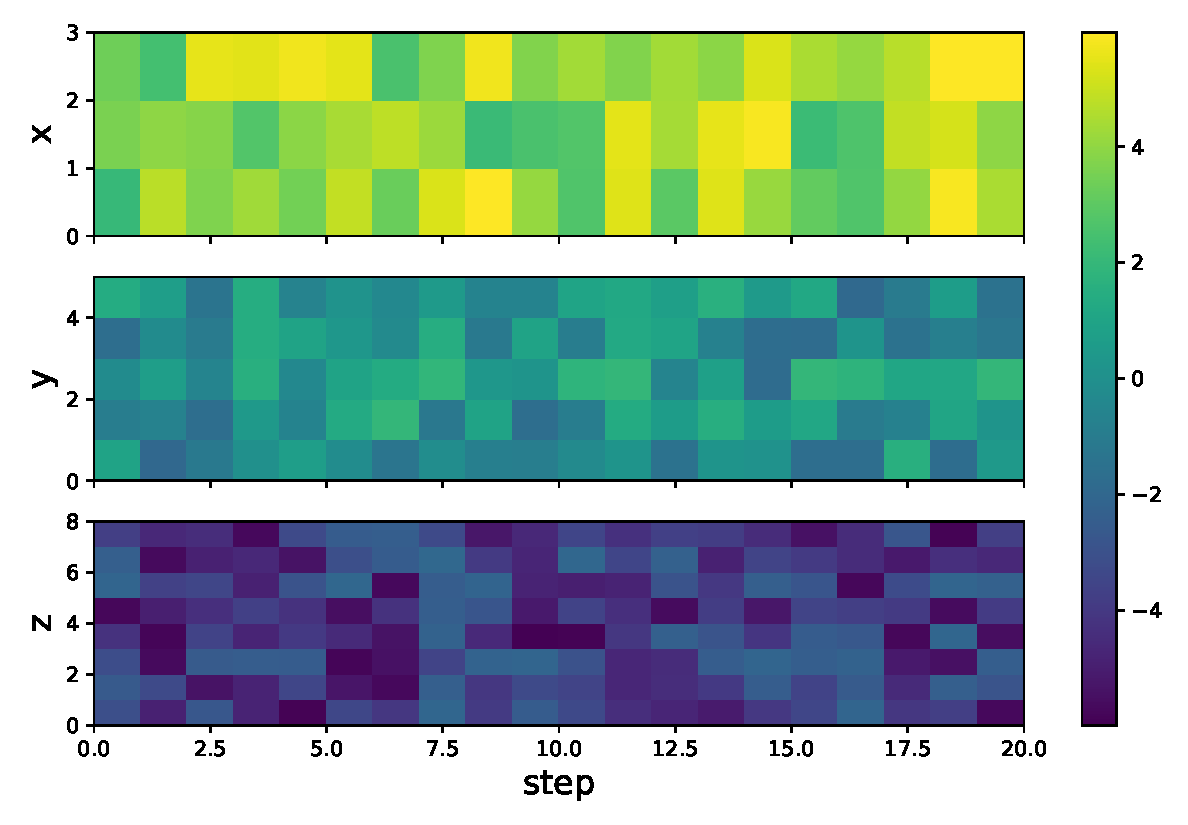
\includegraphics[width=0.9\linewidth]{figs/pcolormesh.eps}
  \caption{pcolormesh}
  \label{fig:pcolormesh}
\end{figure}

条件ごとの結果を\tref{tb:result}に示す.
\begin{table}[htbp]
  \caption{条件ごとの実験結果}
  \label{tb:result}
  \centering\begin{tabular}{c|ccc}\hline
    条件 & loss & acc & std\\\hline
    条件1 & 0.2 & 0.86 & $\pm 0.15$\\\hline
    条件2 & 0.1 & 0.92 & $\pm 0.05$\\\hline
  \end{tabular}
\end{table}

\chapter{議論}
議論を書く.

\chapter{結論}
結論を書く.

\backmatter% ここから後付
\chapter{謝辞}%%%%%%%%%%%%%%% 謝辞 %%%%%%%
謝辞を書く.

% \begin{thebibliography}{}%%%% 参考文献 %%%
%   \bibitem{}
% \end{thebibliography}
\bibliographystyle{junsrt}%           BibTeX を使う場合
\bibliography{bibitem}% BibTeX を使う場合

\appendix% ここから付録 %%%%% 付録 %%%%%%%
\chapter{実験結果の図}
付録があればここに書く.

\end{document}
